\chapter*{Annexe du chapitre \ref{chap:PDZ}}


\label{chap:annexePDZ}
   \begin{figure}[htbp]
     \centering
     \begin{tabular}{c}
       \includegraphics[width=17cm]{homologues/1G9O.png} \\
     \end{tabular}
     \caption{L'alignement de notre sélection de séquences homologues à la protéine NHREF (code PDB: 1G9O)}
\label{align_homo:NHREF}
   \end{figure}

   \begin{figure}[!htbp]
     \centering
     \begin{tabular}{c}
       \includegraphics[width=17cm]{proteus/1G9O.png} \\
     \end{tabular}
       \caption{Une sélection de séquences proteus, parmi les 10 000 séquences de meilleure énergie, obtenues avec le backbone de la protéine NHREF (code PDB: 1G9O), modèle NEA}
\label{align_proteus:NHREF}
   \end{figure}

\clearpage

   \begin{figure}[!htbp]
     \centering
     \begin{tabular}{c}
       \includegraphics[width=17cm]{homologues/1IHJ.png} \\
     \end{tabular}
     \caption{L'alignement de notre sélection de séquences homologues à la protéine INAD (code PDB: 1IHJ )}
\label{align_homo:INAD}
   \end{figure}

   \begin{figure}[!htbp]
     \centering
     \begin{tabular}{c}
       \includegraphics[width=17cm]{proteus/1IHJ.png} \\
     \end{tabular}
       \caption{Une sélection de séquences proteus, parmi les 10 000 séquences de meilleure énergie, obtenues avec le backbone de la protéine INAD (code PDB: 1IHJ), modèle NEA}
\label{align_proteus:INAD}
   \end{figure}
\clearpage

   \begin{figure}[!htbp]
     \centering
     \begin{tabular}{c}
       
\includegraphics[width=17cm]{homologues/1R6J.png} \\
     \end{tabular}
     \caption{L'alignement de notre sélection de séquences homologues à la protéine Syntenin (code PDB: 1R6J)}
\label{align_homo:Syntenin}
   \end{figure}

   \begin{figure}[!htbp]
     \centering
     \begin{tabular}{c}
       
\includegraphics[width=17cm]{proteus/1R6J.png} \\
     \end{tabular}
       \caption{Une sélection de séquences proteus, parmi les 10 000 séquences de meilleure énergie, obtenues avec le backbone de la protéine Syntenin (code PDB: 1R6J), modèle NEA}
\label{align_proteus:Syntenin}
   \end{figure}
\clearpage

   \begin{figure}[!htbp]
     \centering
     \begin{tabular}{c}
       \includegraphics[width=17cm]{homologues/1N7E.png} \\
     \end{tabular}
     \caption{L'alignement de notre sélection de séquences homologues à la protéine GRIP (code PDB: 1N7E)}
\label{align_homo:GRIP}
   \end{figure}

   \begin{figure}[!htbp]
     \centering
     \begin{tabular}{c}
       \includegraphics[width=17cm]{proteus/1N7E.png} \\
     \end{tabular}
       \caption{Une sélection de séquences proteus, parmi les 10 000 séquences de meilleure énergie, obtenues avec le backbone de la protéine GRIP (code PDB: 1N7E), modèle NEA}
\label{align_proteus:GRIP}
   \end{figure}
\clearpage

   \begin{figure}[!htbp]
     \centering
     \begin{tabular}{c}
       \includegraphics[width=17cm]{homologues/2BYG.png} \\
     \end{tabular}
     \caption{L'alignement de notre sélection de séquences homologues à la protéine DLG2 (code PDB: 2BYG)}
\label{align_homo:DLG2}
   \end{figure}

   \begin{figure}[!htbp]
     \centering
     \begin{tabular}{c}
       \includegraphics[width=17cm]{proteus/2BYG.png} \\
     \end{tabular}
       \caption{Une sélection de séquences proteus, parmi les 10 000 séquences de meilleure énergie, obtenues avec le backbone de la protéine DLG2 (code PDB: 2BYG), modèle NEA}
\label{align_proteus:DLG2}
   \end{figure}
\clearpage

   \begin{figure}[!htbp]
     \centering
     \begin{tabular}{c}
       \includegraphics[width=17cm]{homologues/3K82.png} \\
     \end{tabular}
     \caption{L'alignement de notre sélection de séquences homologues à la protéine PSD95 (code PDB: 3K82)}
\label{align_homo:PSD95}
   \end{figure}

   \begin{figure}[!htbp]
     \centering
     \begin{tabular}{c}
       \includegraphics[width=17cm]{proteus/3K82.png} \\
     \end{tabular}
       \caption{Une sélection de séquences proteus, parmi les 10 000 séquences de meilleure énergie, obtenues avec le backbone de la protéine PSD95 (code PDB: 3K82), modèle NEA}
\label{align_proteus:PSD95}
   \end{figure}
\clearpage

   \begin{figure}[!htbp]
     \centering
     \begin{tabular}{c}
       \includegraphics[width=17cm]{homologues/TIAM1.png} \\
     \end{tabular}
     \caption{L'alignement de notre sélection de séquences homologues à la protéine Tiam1 (code PDB )}
\label{align_homo:Tiam1}
   \end{figure}
\clearpage   
   \begin{figure}[!htbp]
     \centering
     \begin{tabular}{c}
       \includegraphics[width=17cm]{homologues/CASK.png} \\
     \end{tabular}
     \caption{L'alignement de notre sélection de séquences homologues à la protéine Cask (code PDB)}
   \label{align_homo:CASK}
   \end{figure}
   
\clearpage



%%% Local Variables:
%%% mode: latex
%%% TeX-master: "these"
%%% End:
